\documentclass[10pt]{beamer}

%% Beamer Layout __________________________________________________
\usetheme{metropolis}
\metroset{block=fill}

\resetcounteronoverlays{exx}

% Loading Packages ________________________________________________
\usepackage {MnSymbol}
\usepackage{fancybox}
\usepackage{pifont}
\usepackage{stmaryrd}
\usepackage{gb4e}
\usepackage{graphicx}
\usepackage{tikz, tikz-qtree}
\usepackage{natbib}
\usetikzlibrary{decorations.fractals}
\usepackage{amsmath}
\usepackage{multirow}
\usepackage{multicol}
\usepackage{color}

\definecolor{ggreen}{rgb}{0.0, 0.5, 0.0}
%_________________________________________________________________

\begin{document}

% Title ___________________________

\begin{frame}
\title{Definiteness in Farsi}
%\subtitle{SUBTITLE}
\author{Masoud Jasbi \\ ~ \\ {\small Department of Linguistics} \\ {\small Stanford University} }       	
%	\vspace{1cm}
\date{}
\titlepage

{\scriptsize UCSD \\ SemBabble}
\end{frame}

% THE in English is argued to carry uniqueness that is presuppositional
% In Tehrani Farsi, uniqueness is contributed by -e but the presence or absence of the indefinite determiner decides the status of this uniqueness implication.
% Implications: presupposition triggers do not have to be encoded lexically as such 

% Definiteness ________________________________
\section {\scshape Definiteness}

\begin {frame} {Definiteness}

	\begin {itemize}
	\item Nominals can be classified into:
	\begin {enumerate}
	\item \textsc{Definites}: \alert{the} king of France, Louis, that man, he, their king, etc.
	\item \textsc{Indefinites}: \alert{a} king of France, some man, any man, every man, etc.
	\end {enumerate}
	\item What semantic-pragmatic properties differentiate definites and indefinites? \pause
	\item What are the functions of \alert{the} and \alert{a}?
	\end {itemize}

\end {frame}
\begin {frame} {Theories of Definiteness}

	\begin {enumerate}
	\item \alert{Uniqueness} {\scriptsize \hfill \citep{russell1905denoting, abbott1999support}}
	\item \alert{Familiarity} {\scriptsize \hfill \citep{heim1982semantics, christophersen1939articles, prince1992zpg}}
	\item Salience {\scriptsize \hfill \citep{lewis1979scorekeeping, von1997salience}}
	\item Givenness {\scriptsize \hfill \citep{gundel1993cognitive}}
	\item Accessibility {\scriptsize \hfill \citep{ariel1990accessing, ariel2001accessibility}}
	\end {enumerate}

\end {frame}

\begin {frame} {Uniqueness}

Definites imply the existence and \alert{uniqueness} of their descriptive content. \pause \\ Indefinites imply the existence.

\end {frame}

%\begin {frame} {Uniqueness}
%
%\center \includegraphics[scale=0.20] {cards}
%
%\# \alert{The cat} is cute here. \pause \\
%A cat is cute here.
%
%\end {frame}
%
%\begin {frame} {Uniqueness}
%
%\center \includegraphics[scale=0.20] {dogelephant}
%
%\# \alert{The cat} is cute here. \pause \\
%\# A cat is cute here.
%
%\end {frame}
%
%\begin {frame} {Uniqueness}
%
%\center \includegraphics[scale=0.20] {catdog}
%
%\alert{The cat} is cute here.\pause \\
%? A cat is cute here.
%
%\end {frame}
%
%\begin {frame} {Uniqueness}
%
%Definites imply uniqueness, indefinites don't.
%
%\end {frame}

\begin {frame} {Presuppositionality}

The existence and uniqueness implication of definites is presuppositional; i.e. common ground between the speaker and the addressee. 

\end {frame}

\begin {frame} {Definiteness}

\begin {tabular} {c | c | c|c}
 & Existence & Uniqueness & Presuppositional \\ \hline
Definite & + & + & + \\
Indefinite & + & $-$ & $-$ \\ 
\end {tabular}
\pause
~\\~\\Common definite articles like \emph{the} encode both uniqueness and presuppositionality. \\   

\end {frame}

\begin {frame} {Definiteness in Farsi}

Farsi (Persian) encodes uniqueness and presuppositionality separately. \pause \\ 
Uniqueness is encoded in the clitic -\emph{{\color{red}e}}. \pause\\
Presuppositionality is controlled by the presence or absence of the indefinite determiner \emph{ye}.\\ \pause
This allows the uniqueness morpheme to cross the definite-indefinite boundary. 

\end {frame}

% Persian ________________________________

\section {\scshape Persian}

\begin {frame} {Crosslinguistic Patterns}

\hfill \includegraphics[scale=0.28] {deftypology}

{\footnotesize
\begin {itemize} 
	\item No definite but indefinite article: around 7\% of the languages in WALS.
	\item Persian is among these languages with Japanese, Quechua, and Turkish.
\end {itemize}
				\hfill {\footnotesize \citep{wals-37, wals} }
}
\end {frame}

\begin {frame} {Persian}

	\begin {itemize}
	\item Family: Indo-European $>$ Indo-Iranian $>$ Iranian \pause
	\item Native to: Iran (Farsi), Afghanistan (Dari), Tajikistan (Tajik)
	\item Speakers: $\sim$110 million
	\item I focus on Farsi.
	\end {itemize}

	\hfill \includegraphics[scale=0.2] {persian}

\end {frame}

\begin {frame} {Farsi}

    \begin {itemize}
    \item Varieties: Tehrani, Yazdi, Shirazi, etc. \pause
    \item I focus on Tehrani Farsi.
    \end {itemize}
    
    \hfill \includegraphics[scale=0.25] {tehran}
    
    \end {frame}

\begin {frame} {Definiteness in Persian}

\begin {itemize} 
	\item No article or marker like \emph{the} in English. \pause
	\item Two indefinite markers: 				
	\begin {enumerate} [i.]
		\item The indefinite determiner \emph{ye}.
		\item The indefinite clitic \emph{-i}.
	\end {enumerate} \pause
	\item Two markers that cut across the definite/indefinite classification:
	\begin {enumerate} [i.]
		\item The object marker \emph{-r\={a}}.
		\item The N-clitic \emph{-e}.
	\end {enumerate}
\end {itemize}

\end {frame}
%%%%%%%%%%%%%%%%%%%

\begin {frame} {Nominal Constructions in Persian}

\begin {tabular}{l | r}
\multicolumn{2}{c}{} \\\hline
\hspace{0.44cm}NP & Definite, Generic, Indefinite\\ \hline
\hspace{0.44cm}N-{\color {red}e} & Definite \\ \hline
{\color {ggreen}ye}-NP & Simple Indefinite\\ \hline
\hspace{0.44cm}NP-{\color {blue}i} & Antidefinite\\ \hline
{\color {ggreen}ye}-N-{\color {red}e} & Singleton Indefinite\\ \hline
{\color {ggreen}ye}-NP-{\color {blue}i} & Complex Indefinite\\ \hline
%\multicolumn{2}{c}{Non-direct-object Positions} \\\hline
%\hspace{0.44cm}NP-\textbf{r\={a}} & Definite, Generic, Indefinite Object\\ \hline
%\hspace{0.44cm}N-{\color {red}e}-\textbf{r\={a}} & Definite Object\\ \hline
%{\color {ggreen}ye}-NP-\textbf{r\={a}} & Simple Indefinite Object\\ \hline
%\hspace{0.44cm}NP-{\color {blue}i}-\textbf{r\={a}} & Antidefinite Object\\ \hline
%{\color {ggreen}ye}-N-{\color {red}e}-\textbf{r\={a}} & Singleton Indefinite Object\\ \hline
%{\color {ggreen}ye}-NP--{\color {blue}i}-\textbf{r\={a}} & Complex Indefinite Object\\
\end {tabular}

\end {frame}
%%%%%%%%%%%%%%%%%%%

\begin {frame} {Nominal Constructions in Persian}

\begin {tabular}{l | r}
%\multicolumn{2}{c}{Non-direct-object Positions} \\\hline
%\hspace{0.44cm}NP & Definite, Generic, Indefinite\\ \hline
%\hspace{0.44cm}N-{\color {red}e} & Definite \\ \hline
%{\color {ggreen}ye}-NP & Simple Indefinite\\ \hline
%\hspace{0.44cm}NP-{\color {blue}i} & Antidefinite\\ \hline
%{\color {ggreen}ye}-N-{\color {red}e} & Singleton Indefinite\\ \hline
%{\color {ggreen}ye}-NP-{\color {blue}i} & Complex Indefinite\\ \hline
\multicolumn{2}{c}{Direct-Object Position} \\\hline
\hspace{0.44cm}NP-\textbf{r\={a}} & Definite, Generic, Indefinite Object\\ \hline
\hspace{0.44cm}N-{\color {red}e}-\textbf{r\={a}} & Definite Object\\ \hline
{\color {ggreen}ye}-NP-\textbf{r\={a}} & Simple Indefinite Object\\ \hline
\hspace{0.44cm}NP-{\color {blue}i}-\textbf{r\={a}} & Antidefinite Object\\ \hline
{\color {ggreen}ye}-N-{\color {red}e}-\textbf{r\={a}} & Singleton Indefinite Object\\ \hline
{\color {ggreen}ye}-NP--{\color {blue}i}-\textbf{r\={a}} & Complex Indefinite Object\\\hline
\end {tabular}

\end {frame}
%%%%%%%%%%%%%%%%%%%

\begin {frame} {Nominal Constructions in Persian}

\begin {tabular}{l | r}
\multicolumn{2}{c}{} \\\hline
\hspace{0.44cm}NP & Definite, Generic, Indefinite\\ \hline
\hspace{0.44cm}N-{\color {red}e} & Definite \\ \hline
{\color {ggreen}ye}-NP & Simple Indefinite\\ \hline
\hspace{0.44cm}NP-{\color {blue}i} & Antidefinite\\ \hline
{\color {ggreen}ye}-N-{\color {red}e} & Singleton Indefinite\\ \hline
{\color {ggreen}ye}-NP-{\color {blue}i} & Complex Indefinite\\ \hline
%\multicolumn{2}{c}{Non-direct-object Positions} \\\hline
%\hspace{0.44cm}NP-\textbf{r\={a}} & Definite, Generic, Indefinite Object\\ \hline
%\hspace{0.44cm}N-{\color {red}e}-\textbf{r\={a}} & Definite Object\\ \hline
%{\color {ggreen}ye}-NP-\textbf{r\={a}} & Simple Indefinite Object\\ \hline
%\hspace{0.44cm}NP-{\color {blue}i}-\textbf{r\={a}} & Antidefinite Object\\ \hline
%{\color {ggreen}ye}-N-{\color {red}e}-\textbf{r\={a}} & Singleton Indefinite Object\\ \hline
%{\color {ggreen}ye}-NP--{\color {blue}i}-\textbf{r\={a}} & Complex Indefinite Object\\
\end {tabular}

\end {frame}
%%%%%%%%%%%%%%%%%%%

\begin {frame} {Focus of This Project}

\begin {tabular}{l | r}
\multicolumn{2}{c}{} \\\hline
\hspace{0.44cm}N & Definite, Generic, Indefinite\\ \hline
\hspace{0.44cm}N-{\color {red}e} & Definite \\ \hline
{\color {ggreen}ye}-NP & Simple Indefinite\\ \hline
%\hspace{0.44cm}NP-{\color {blue}i} & Antidefinite\\ \hline
{\color {ggreen}ye}-N-{\color {red}e} & Singleton Indefinite\\ \hline
%{\color {ggreen}ye}-NP-{\color {blue}i} & Complex Indefinite\\ \hline
%\multicolumn{2}{c}{Non-direct-object Positions} \\\hline
%\hspace{0.44cm}NP-\textbf{r\={a}} & Definite, Generic, Indefinite Object\\ \hline
%\hspace{0.44cm}N-{\color {red}e}-\textbf{r\={a}} & Definite Object\\ \hline
%{\color {ggreen}ye}-NP-\textbf{r\={a}} & Simple Indefinite Object\\ \hline
%\hspace{0.44cm}NP-{\color {blue}i}-\textbf{r\={a}} & Antidefinite Object\\ \hline
%{\color {ggreen}ye}-N-{\color {red}e}-\textbf{r\={a}} & Singleton Indefinite Object\\ \hline
%{\color {ggreen}ye}-NP--{\color {blue}i}-\textbf{r\={a}} & Complex Indefinite Object\\
\end {tabular}
\pause
\begin {itemize} 
	\item What does \emph{-{\color {red}e}} do?
\end {itemize}

\end {frame}
%%%%%%%%%%%%%%%%%%%

\section {\scshape Empirical Observations}

\begin {frame} {Nominal Constructions}

\begin {tabular}{l | r}
\multicolumn{2}{c}{} \\\hline
\alert{\hspace{0.44cm}N} & \alert{Definite, Generic, Indefinite}\\ \hline
\hspace{0.44cm}N-{\color {red}e} & Definite \\ \hline
{\color {ggreen}ye}-NP & Simple Indefinite\\ \hline
{\color {ggreen}ye}-N-{\color {red}e} & Singleton Indefinite\\ \hline
\end {tabular}

\end {frame}
%%%%%%%%%%%%%%%%%%%

\begin {frame} {Bare Nominals}

\begin {exampleblock} {Generic Example}
{\small C_{Gen}: Amir is discussing cars and their problems. He says:}
	\begin {exe}
		\ex \label{bache} \gll	m\={a}shin	hav\={a}-ro	\={a}lude	mi-kon-e\\
			car	air-{\scriptsize -OM}	polluted	{\scriptsize MI-}do{\scriptsize -3.SG}\\
			``Cars pollute the air.''\\
	\end {exe}
\end {exampleblock}

\pause

\begin {exampleblock} {Indefinite Example}
{\small C_{indef}: Amir is crossing the street without checking the traffic. Leila stops him and says: }
	\begin {exe}
		\ex \label{} \gll	m\={a}shin	mi-zan-e be-het\\
			car	{\scriptsize MI-}hit{\scriptsize -3.SG} to-{\scriptsize -2.SG}\\
			``A car is gonna hit you.''\\
	\end {exe}

\end {exampleblock}

\end {frame}

\begin {frame} {Bare Nominals}

\begin {exampleblock} {Definite Example}
{\small C_{def_1}: Amir and Leila have one car only. One day Amir comes home and says:}
	\begin {exe}
		\ex \label{} \gll	m\={a}shin	xar\={a}b	shod-e\\
			car	broken	become{\scriptsize .PST-3.SG}\\
			``The car's broken.''\\
	\end {exe}
\end {exampleblock}
\pause
    \begin {exampleblock} {Definite Example}
{\small C_{def_2}: Early in the morning, Leila says:}
    	\begin {exe}
    		\ex \label{} \gll	xorshid	dar-umad\\
    			sun	out-come{\scriptsize .3.SG}\\
    			``The sun came out.''\\
    	\end {exe}
    \end {exampleblock}
\end {frame}

\begin {frame} {Bare Nominals}
Bare Nominals in Tehrani Farsi can be definite, indefinite, or generic.
\end {frame}

\begin {frame} {Nominal Constructions}

\begin {tabular}{l | r}
\multicolumn{2}{c}{} \\\hline
\hspace{0.44cm}N & Definite, Generic, Indefinite\\ \hline
\alert{\hspace{0.44cm}N-{\color {red}e}} & \alert{Definite} \\ \hline
{\color {ggreen}ye}-NP & Simple Indefinite\\ \hline
{\color {ggreen}ye}-N-{\color {red}e} & Singleton Indefinite\\ \hline
\end {tabular}

\end {frame}
%%%%%%%%%%%%%%%%%%%

\begin {frame} {N-\emph{{\color {red}e}}}

\begin {exampleblock} {N}
{\small C_{Gen}: Amir is discussing cars and their problems. He says:}
	\begin {exe}
		\ex \label{} \gll	m\={a}shin	hav\={a}-ro	\={a}lude	mi-kon-e\\
			car	air-{\scriptsize -OM}	polluted	{\scriptsize MI-}do{\scriptsize -3.SG}\\
			``Cars pollute the air.''\\
	\end {exe}
\end {exampleblock}

\pause

\begin {exampleblock} {N-{\color {red}e}}
{\small {\color {gray}\#C_{Gen}}}
{\small C_{def_3}: Amir shows the video of an old car with a smokey exhaust. He says:}

	\begin {exe}
		\ex \label{} \gll	m\={a}shin-\emph{{\color {red}e}}	hav\={a}-ro	\={a}lude	mi-kon-e\\
			car-{\scriptsize UM}	air-{\scriptsize -OM}	polluted	{\scriptsize MI-}do{\scriptsize -3.SG}\\
			``The/that car pollutes the air.''\\
	\end {exe}
\end {exampleblock}

\end {frame}

%%%%%%%%%%%%%%%%%%%
\begin {frame} {N-\emph{{\color {red}e}}}

\begin {exampleblock} {N}
{\small C_{indef}: Amir is crossing the street without checking the traffic. Leila stops him and says: }
	\begin {exe}
		\ex \label{} \gll	m\={a}shin	mi-zan-e be-het\\
			car	{\scriptsize MI-}hit{\scriptsize -3.SG} to-{\scriptsize -2.SG}\\
			``A car is gonna hit you.''\\
	\end {exe}

\end {exampleblock}

\pause

\begin {exampleblock} {N-{\color {red}e}}
{\small {\color {gray}\#C_{indef} }}
{\small C_{def_4}: Amir is walking in a parking lot. A car is backing out. Leila stops him and says: }
	\begin {exe}
		\ex \label{} \gll	m\={a}shin-\emph{{\color {red}e}}	mi-zan-e be-het\\
			car-{\scriptsize UM}	{\scriptsize MI-}hit{\scriptsize -3.SG} to-{\scriptsize -2.SG}\\
			``The/that car is gonna hit you.''\\
	\end {exe}

\end {exampleblock}

\end {frame}

%%%%%%%%%%%%%%%%%%%

\begin {frame} {N-\emph{{\color {red}e}}}

\begin {exampleblock} {N}
{\small C_{def_1}: Amir and Leila have one car only. One day Amir comes home and says:}
	\begin {exe}
		\ex \label{} \gll	m\={a}shin	xar\={a}b	shod-e\\
			car	broken	become{\scriptsize .PST-3.SG}\\
			``The car's broken.''\\
	\end {exe}
\end {exampleblock}
\pause
\begin {exampleblock} {N-\emph{{\color {red}e}}}
{\small C_{def_1}}
	\begin {exe}
		\ex \label{} \gll	m\={a}shin-\emph{{\color {red}e}}	xar\={a}b	shod-e\\
			car-{\scriptsize UM}	broken	become{\scriptsize .PST-3.SG}\\
			``The/that car's broken.''\\
	\end {exe}
\end {exampleblock}

\end {frame}

%%%%%%%%%%%%%%%%%%%

\begin {frame} {N-\emph{{\color {red}e}}}

\begin {exampleblock} {N}
{\small C_{def_2}: Early in the morning, Leila says:}
	\begin {exe}
		\ex \label{bache} \gll	xorshid-\emph{{\color {red}e}}	dar-umad\\
			sun-{\scriptsize UM}	out-come{\scriptsize .3.SG}\\
			``The sun came out.''\\
	\end {exe}
\end {exampleblock}
\pause
\begin {exampleblock} {N-\emph{{\color {red}e}}}
{\small C_{def_2}}
	\begin {exe}
		\ex \label{bache} \gll	xorshid-\emph{{\color {red}e}}	dar-umad\\
			sun-{\scriptsize UM}	out-come{\scriptsize .3.SG}\\
			``The/that sun came out.''\\
	\end {exe}
\end {exampleblock}

\end {frame}

%%%%%%%%%%%%%%%%%%%

\begin {frame} {Summary}
Adding -{\color {red}e} to a bare nominal makes it (definitely) definite. \\
\end {frame}

\begin {frame} {Nominal Constructions}

\begin {tabular}{l | r}
\multicolumn{2}{c}{} \\\hline
\hspace{0.44cm}N & Definite, Generic, Indefinite\\ \hline
\hspace{0.44cm}N-{\color {red}e} & Definite \\ \hline
\alert{ye-N} & \alert{Simple Indefinite}\\ \hline
\alert{ye-N-{\color {red}e}} & \alert{Singleton Indefinite}\\ \hline
\end {tabular}

\end {frame}
%%%%%%%%%%%%%%%%%%%

\begin {frame} {(ye) N-\emph{{\color {red}e}}}

\begin {exampleblock} {ye N}
{\small C_{indef}: Leila looks out the window. She says:}
	\begin {exe}
		\ex \label{} \gll	ye zan dam-e dar-e\\
					{\scriptsize Indef.D} woman close-{\scriptsize EZ} door-{\scriptsize 3.SG}\\
			``A woman is at the door.''\\
	\end {exe}
\end {exampleblock}
\pause
\begin {exampleblock} {ye N-\emph{{\color {red}e}}}
{\small C_{indef}: Leila looks out the window. She says:}
	\begin {exe}
		\ex \label{} \gll	ye zan-{\color{red}e} dam-e dar-e\\
					{\scriptsize Indef.D} woman-{\scriptsize UM} close-{\scriptsize EZ} door-{\scriptsize 3.SG}\\
			``A woman is at the door.''\\
	\end {exe}
\end {exampleblock}

\end {frame}

%%%%%%%%%%%%%%%%%%%

\begin {frame} {Nominal Constructions}

What is the difference between ye-N and ye-N-{\color {red}e}? \\ \pause
Answer: mainly scope.

\end {frame}
%%%%%%%%%%%%%%%%%%%

\begin {frame} {De-re De-dicto}

\begin {exampleblock} {ye N}
	\begin {exe}
		\ex \label{} \gll	Amir mi-x\={a}-d b\={a} ye doxtar ezdev\={a}j kon-e\\
					Amir {\scriptsize MI}-want-{\scriptsize 3.SG} with {\scriptsize In.D} girl marry do-{\scriptsize 3.SG}\\
			``Amir wants to marry a girl.'' \\ \pause 1. $\exists > \textsc{want}$ \\2. $\textsc{want} > \exists$\\
	\end {exe}
\end {exampleblock}
\pause
\begin {exampleblock} {ye N-\emph{{\color {red}e}}}
	\begin {exe}
		\ex \label{} \gll	Amir mi-x\={a}-d b\={a} ye doxtar-{\color {red}e} ezdev\={a}j kon-e\\
					Amir {\scriptsize MI}-want-{\scriptsize 3.SG} with {\scriptsize In.D} girl-{\scriptsize UM} marry do-{\scriptsize 3.SG}\\
			``Amir wants to marry a girl.'' \\ 1. $\exists > \textsc{want}$\\
	\end {exe}
\end {exampleblock}

\end {frame}

%%%%%%%%%%%%%%%%%%%

\begin {frame} {Scope with the Universal Quantifier}

\begin {exampleblock} {ye N}
	\begin {exe}
		\ex \label{} \gll	emruz hame be ye ost\={a}d sal\={a}m kard-im\\
					today everyone to {\scriptsize Indef.D} professor hello do-{\scriptsize 1.PL}\\
			``Today everyone said hello to a professor.'' \\ \pause 1. $\exists > \forall$ \\ 2. $\forall > \exists$ 2. \\
	\end {exe}
\end {exampleblock}
\pause
\begin {exampleblock} {ye N-\emph{{\color {red}e}}}
	\begin {exe}
		\ex \label{} \gll	emruz hame be ye ost\={a}d-{\color {red} e} sal\={a}m kard-im\\
					today everyone to {\scriptsize Indef.D} professor-{\scriptsize UM} hello do-{\scriptsize 1.PL}\\
			``Today everyone said hello to a specific professor.'' \\ 1. $\exists > \forall$\\
	\end {exe}
\end {exampleblock}

\end {frame}

%%%%%%%%%%%%%%%%%%%

\begin {frame} {Scope with the Universal Quantifier}

\begin {exampleblock} {ye N}
{\footnotesize
	\begin {exe}
		\ex \label{} \gll	har doxtar hame-ye eshteb\={a}-h\={a}-ye ye pesar ro tasih kard\\
					each girl	every-{\scriptsize EZ} mistake-{\scriptsize PL}-{\scriptsize EZ} {\scriptsize Indef.D} boy {\scriptsize OM} correct do-{\scriptsize 1.PL}\\
			``Every girl corrected all the mistakes of a boy.'' \\ \pause 1. $ \exists > \forall > \forall$ \\ 2. $\forall > \exists > \forall$\\
	\end {exe}}
\end {exampleblock}
\pause
\begin {exampleblock} {ye N-\emph{{\color {red}e}}}
{\footnotesize
	\begin {exe}
		\ex \label{} \gll	har doxtar hame-ye eshteb\={a}-h\={a}-ye ye pesar-{\color {red}e} ro tasih kard\\
					each girl	every-{\scriptsize EZ} mistake-{\scriptsize PL}-{\scriptsize EZ} {\scriptsize Indef.D} boy-{\scriptsize UM} {\scriptsize OM} correct do-{\scriptsize 1.PL}\\
			``There is a boy that every girl corrected all his mistakes.'' \\ 1. $ \exists > \forall > \forall$\\
	\end {exe}}
\end {exampleblock}

\end {frame}

%%%%%%%%%%%%%%%%%%%

\begin {frame} {Scope with Temporal Adverbials}

\begin {exampleblock} {ye N}
{\footnotesize
	\begin {exe}
		\ex \label {} \gll	S\={a}r\={a}	hamishe		b\={a}	ye pesar		dav\={a}-sh	mi-sh-e\\
				Sara	always 	with		{\scriptsize Indef.D} boy	quarrel{\scriptsize -3.SG}	{\scriptsize MI-}become{\scriptsize -3.SG}\\
			``Sara always gets into a fight with some boy.'' \\ \pause 1. $\exists > \textsc{always}$ \\ 2. $\textsc{always} > \exists $\\
	\end {exe}}
\end {exampleblock}
\pause
\begin {exampleblock} {ye N-\emph{{\color {red}e}}}
{\footnotesize
	\begin {exe}
		\ex \label {} \gll	S\={a}r\={a}	hamishe		b\={a}	ye pesar{\color {red}-e}		dav\={a}-sh	mi-sh-e\\
				Sara	always 	with		{\scriptsize Indef.D} boy({\scriptsize -UM})	quarrel{\scriptsize -3.SG}	{\scriptsize MI-}become{\scriptsize -3.SG}\\
			``Sara always gets into a fight with some boy.'' \\ 1. $\exists > \textsc{always}$
	\end {exe}}
\end {exampleblock}

\end {frame}

%%%%%%%%%%%%%%%%%%%

\begin {frame} {Summary}
Adding -{\color {red}e} to a bare nominal makes it (definitely) definite. \\
Adding -{\color {red}e} to an indefinite enforces a widest scope reading.
\end {frame}

\begin {frame} {Specificity?}

Does -{\color {red}e} make an indefinite specific in the sense of Fodor \& Sag (1982)? \\
Does ye-N-{\color {red}e} require the speaker to have a specific referent in mind? \pause

\begin {exampleblock} {Examples}
	\begin {exe}
		\ex \label{} \gll	dust-am eshteb\={a}hi eskirin-sh\={a}t-e chat-esh-o b\={a} ye doxtar-{\color{red}e} ferest\={a}d \\
			friend-{\scriptsize 1.SG} mistakenly screen-shot-{\scriptsize EZ}	chat-{\scriptsize 3.SG-OM} with {\scriptsize In.D}	girl-{\scriptsize UM} sent{\scriptsize .3.SG}\\
			``My friend mistakenly sent me a screen shot of his chat with a girl.''  \\
	\end {exe}
\end {exampleblock}

\end {frame}

\begin {frame} {Summary}
Adding -{\color {red}e} to a bare nominal makes it (definitely) definite. \\
Adding -{\color {red}e} to an indefinite enforces a widest scope reading. \\ \pause
What meaning for -{\color {red}e} can result in both these effects? \\
\end {frame}

\section {\scshape A Proposal}

\begin {frame} {Proposal}
The clitic -{\color {red}e} encodes a uniqueness implication. \\ \pause
Adding it to a bare nominal makes it definite. \\ \pause
Adding to an indefinite results in a singleton indefinite, making scope relations inert (Schwarzschild 2002). \\ \pause
Is the uniqueness implication cancellable by entailment canceling operators like negation or conditional antecedents? 
\end {frame}

\begin {frame} {Negation}

\begin {exampleblock} {ye N}
	\begin {exe}
		\ex \label{} \gll	Rez\={a} b\={a} ye doxtar ham na-raqsid\\
			Reza with {\scriptsize In.D} girl even {\scriptsize NEG}-danced{\scriptsize .3.SG}\\
			``Reza did not dance with any girl.'' ($\lnot > \exists$) \\ \pause $\not \rightsquigarrow$ ``There is a girl.''
	\end {exe}
\end {exampleblock}
\pause
\begin {exampleblock} {ye N-\emph{{\color {red}e}}}
	\begin {exe}
		\ex \label{} \gll	Rez\={a} b\={a} ye doxtar-{\color {red}e} ham na-raqsid\\
			Reza with {\scriptsize In.D} girl-{\scriptsize UM} even {\scriptsize NEG}-danced{\scriptsize .3.SG}\\
			``There was a girl Reza did not dance with.'' ($\exists > \lnot$) \\ \pause $\rightsquigarrow$ ``There is a unique girl.''
	\end {exe}
\end {exampleblock}

\end {frame}

%%%%%%%%%%%%%%%%%%%

\begin {frame} {Antecedent of Conditionals}

\begin {exampleblock} {ye N}
	\begin {exe}
		\ex \label{} \gll	age b\={a}	ye taksh\={a}x	dust		bud-am, \={a}li bud\\
			if with {\scriptsize In.D}	unicorn	friend was-{\scriptsize 1.SG},	great was{\scriptsize .1.SG}\\
			``It would've been great, If I was friends with a unicorn.'' \\ \pause $\not \rightsquigarrow$ ``There is a unicorn.''
	\end {exe}
\end {exampleblock}
\pause
\begin {exampleblock} {ye N-\emph{{\color {red}e}}}
	\begin {exe}
		\ex \label{} \gll	age b\={a}	ye taksh\={a}x-{\color {red}e}	dust		bud-am, \={a}li bud\\
			if with {\scriptsize In.D}	unicorn-{\scriptsize UM}	friend was-{\scriptsize 1.SG},	great was{\scriptsize .1.SG}\\
			``It would've been great, If I was friends with a unicorn.'' \\ $\not \rightsquigarrow$ ``There is a unique unicorn.''
	\end {exe}
\end {exampleblock}

\end {frame}

\begin {frame} {Proposal}
The clitic -{\color {red}e} encodes a uniqueness implication. \\ 
The uniqueness implication is projective. \\ \pause
Is it the result of constraints on the common ground?
\end {frame}

%%%%%%%%%%%%%%%%%%%

\begin {frame} {Strong Contextual Felicity}

\begin {block}{Definition}
\textsc{m-positive context}: an utterance context that entails or implies $m$.
\textsc{m-neutral context}: an utterance context that entails or implies neither m nor $\lnot$m.
\end {block} 

\begin {exampleblock} {Example}
$C_{Tehrani}$: \{The Tehrani family lives in Tehran, they have one son\}\\
$C_{Yazdi}$: \{The Yazdi family lives in Yazd.\}\\

$m$: there is exactly one son.\\
%$m_{dtr}$: there is only one daughter.\\
~\\
$C_{Tehrani}$ $\Rightarrow$ $m$ \hfill $C_{Tehrani}$ is $m$-positive\\
$C_{Yazdi}$ $\not \Rightarrow$ $m$, $C_{Yazdi}$ $\not \Rightarrow$ $\lnot m$ \hfill  $C_{Yazdi}$ is $m$-neutral
\end {exampleblock}

\end {frame}

%%%%%%%%%%%%%%%%%%%
\begin {frame}{Strong Contextual Felicity}

\begin {block} {Definition}
\textsc{strong contextual felicity constraint}: If utterance of trigger \emph{t} of projective content \emph{m} is acceptable only in an m-positive context, then \emph{t} imposes a strong contextual felicity constraint with respect to m.
\end {block}
\pause
\begin {exampleblock}{Example}
\begin {tabular}{c | c | c | c | c}
$t$ & $m$ & contexts & status & judgement \\ \hline
\multirow{2}{*}{-\emph{e}}& \multirow{2}{*}{there is exactly one son} & $C_{Tehrani}$ & m-positive & $\checkmark$ \\ 
& & $C_{Yazdi}$ & m-neutral & \# \\
\end {tabular}
\end {exampleblock}

\end {frame}

%%%%%%%%%%%%%%%%%%%%

\begin {frame}{Strong Contextual Felicity}

\begin {exampleblock} {m-Positive Context}
In the Tehrani family, \dots
	\begin {exe}
		\ex \label {tehrani} 
			\gll 	pesar-{\color{blue}e}	ezdev\={a}j kard-e \\
				son-e	marry do-{\scriptsize PERF.3.SG}\\
			\glt 	``The son has married."
	\end {exe}
\end {exampleblock}
\pause
\begin {exampleblock} {m-Netural Context}
In the Yazdi family, \dots
	\begin {exe}
		\ex \label {tehrani} 
			\gll 	\# pesar-{\color{blue}e}	ezdev\={a}j kard-e \\
				{} son-e	marry do-{\scriptsize PERF.3.SG}\\
			\glt 	``The son has married."
	\end {exe}
\end {exampleblock}

\end {frame}

%%%%%%%%%%%%%%%%%%%%

\begin {frame}{Strong Contextual Felicity}

\begin {exampleblock} {m-Positive Context}
In the Tehrani family, \dots
	\begin {exe}
		\ex \label {tehrani} 
			\gll 	\# {\color{red} ye} 		pesar-{\color{blue}e}	ezdev\={a}j kard-e \\
				{}	In.D	son-e	marry do-{\scriptsize PERF.3.SG}\\
			\glt 	``A son has married."
	\end {exe}
\end {exampleblock}
\pause
\begin {exampleblock} {m-Netural Context}
In the Yazdi family, \dots
	\begin {exe}
		\ex \label {tehrani} 
			\gll 	{\color{red} ye} pesar-{\color{blue}e}	ezdev\={a}j kard-e \\
				In.D	son-e	marry do-{\scriptsize PERF.3.SG}\\
			\glt 	``A son has married."
	\end {exe}
\end {exampleblock}

\end {frame}

%%%%%%%%%%%%%%%%%%%%

\begin {frame} {Summary}

-{\color {red}e} carries a projective uniqueness implication. \\ \pause
The indefinite determiner \emph{ye} determines if this implication is presuppositional.\\

\end {frame}
%%%%%%%%%%%%%%%%%%%

\section {\scshape Formal Analysis}

\begin {frame} {Analysis}

How can we implement these intuitions formally?

\end {frame}

\begin {frame} {Bare Nominal}

\begin {center}
{\small
	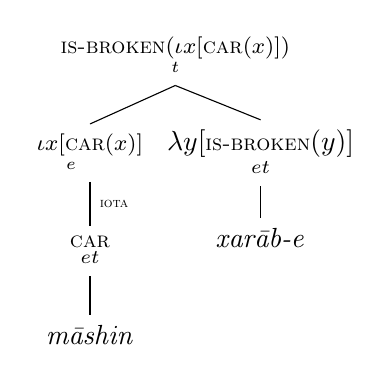
\begin{tikzpicture}[level distance=35pt]
	\Tree [.{\footnotesize$\underset{t}{\footnotesize\textsc{is-broken} (\iota x [ \textsc{car}(x)])}$}
				[.{\footnotesize $\underset{e}{\iota x [\textsc{car}}(x)]$} \edge node[auto=left] {\tiny \textsc{iota}}; [.{$\underset{et}{\footnotesize\textsc{car}}$} [.\emph{m\={a}shin} ] ] ]
        		[.{$\footnotesize \underset{et}{\lambda y [\textsc{is-broken} (y)]}$} [.\emph{xar\={a}b-e} ]
        		]
			]
	\end{tikzpicture}	
}\end {center}

\end {frame}
%%%%%%%%%%%%%%%%%%%%%%

\begin {frame} {Simple Indefinte (ye N)}

\begin {center}
{\small
	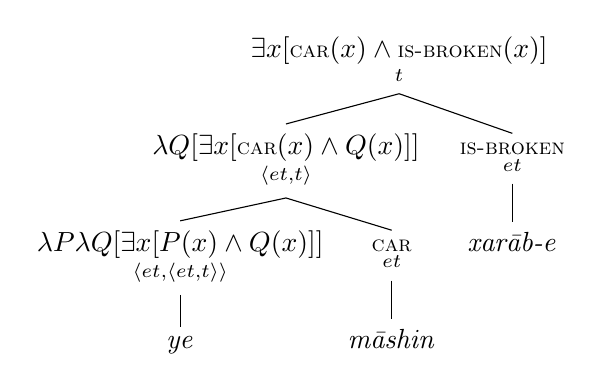
\begin{tikzpicture}[level distance=35pt]
	\Tree [.{$\underset{t}{\footnotesize \exists x [\textsc{car}(x) \land \textsc{is-broken} (x)]}$}
				[.{$\underset{\langle et,t\rangle}{\footnotesize\lambda Q [\exists x [\textsc{car}(x) \land Q (x)]]}$}
			[.{$\underset{\langle et, \langle et,t\rangle \rangle}{\footnotesize \lambda P \lambda Q [\exists x [P(x) \land Q (x)]]}$} [.\emph{ye} ] ]
    		[.{$\underset{et}{\footnotesize \textsc{car}}$} [.\emph{m\={a}shin} ] ]
    			]
        		[.{$\underset{et}{\footnotesize\textsc{is-broken}}$} [.\emph{xar\={a}b-e} ]
        		]
			]
	\end{tikzpicture}	
} 
\end {center}

\end {frame}
%%%%%%%%%%%%%%%%%%%%%%

\begin {frame} {Singleton Indefinite (ye N-e)}

\begin {center}
{\small
	\begin {tikzpicture}[level distance=35pt]
	\Tree [.{\footnotesize $\underset{t ~\bullet ~t^c}{\exists x [\textsc{car}(x) \land \textsc{is-broken} (x)] \bullet |\textsc{car}| = 1}$}
				[.{\footnotesize$\underset{\langle et,t\rangle ~\bullet ~t^c}{\lambda Q [\exists x [\textsc{car}(x) \land Q (x)]] \bullet |\textsc{car}| = 1}$}
			[.{\footnotesize$\underset{\langle et, \langle et,t\rangle \rangle}{\lambda P \lambda Q [\exists x [P(x) \land Q (x)]] }$} [.\emph{ye} ] ]
    		[.{\footnotesize$\underset{et ~\bullet ~t^c}{\textsc{car} \bullet |\textsc{car}| = 1}$} 
			[.{\footnotesize$\underset{et}{\textsc{car}}$}  [.\emph{m\={a}shin} ] ] \edge node[auto=left] {\tiny \textsc{CI Application}};
    		[.{\footnotesize$\underset{\langle et, t^c \rangle}{\lambda P [|P| = 1]}$}   [.\emph{-e} ] ] 	
		] 
			]
        		[.{\footnotesize$\underset{et}{\textsc{is-broken}}$} [.\emph{xar\={a}b-e} ] ]
		]
	\end{tikzpicture}	
}
\end {center}

\end {frame}

\begin {frame} {Definite (N-e)}

\begin {center}
{\small
	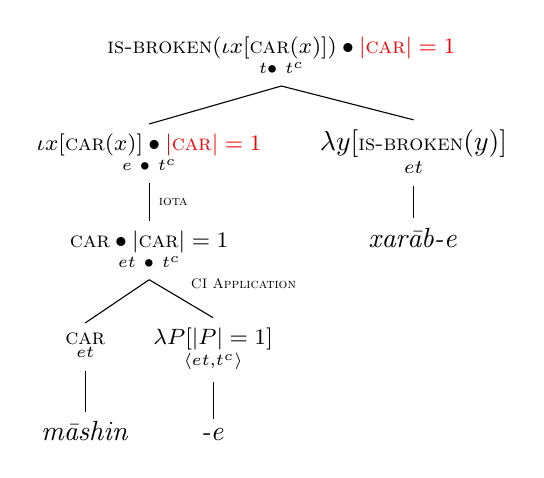
\begin{tikzpicture}[level distance=35pt]
	\Tree [.{\footnotesize$\underset{t \bullet ~t^c}{\footnotesize\textsc{is-broken} (\iota x [ \textsc{car}(x)]) \bullet {\color {red}|\textsc{car}| = 1}}$}
				[.{\footnotesize $\underset{e~\bullet ~t^c}{\iota x [\textsc{car}(x)] \bullet {\color {red}|\textsc{car}| = 1}}$} \edge node[auto=left] {\tiny \textsc{iota}}; 
				[.{\footnotesize$\underset{et ~\bullet ~t^c}{\textsc{car} \bullet |\textsc{car}| = 1}$} 
			[.{\footnotesize$\underset{et}{\textsc{car}}$}  [.\emph{m\={a}shin} ] ] \edge node[auto=left] {\tiny \textsc{CI Application}};
    		[.{\footnotesize$\underset{\langle et, t^c \rangle}{\lambda P [|P| = 1]}$}   [.\emph{-e} ] ] 	
		]				
				]
        		[.{$\footnotesize \underset{et}{\lambda y [\textsc{is-broken} (y)]}$} [.\emph{xar\={a}b-e} ]
        		]
			]
	\end{tikzpicture}	
}\end {center}

\end {frame}
%%%%%%%%%%%%%%%%%%%%%%

\begin {frame} {thank you!} 
\begin {itemize}
\item An indefinite number of thanks to: 
\begin {itemize}
\item Leila Habibi. 
\item Cleo Condoravdi for continued help and support with this project.
\end {itemize}
\end {itemize}
\end {frame} 

%%%%%%%%%%%%%%%%%%%%

\begin {frame} {References} 
\bibliographystyle{apalike}
\bibliography{/Users/Masoud/Google/Academia/Bibliography.bib}
\end {frame} 

\end{document}